% !TeX root = ../master.tex

\lecture{1}{2026-08-25}{Fibermaterialer, pt. I}

\section{Introduktion til kompositter}
Kompositter er kombinationer af to eller flere materialer der er sat sammen med et bindemiddel.
På den vis er både mennesker, huse og træer i og for sig kompositter.
Der findes enormt mange forskellige typer, herunder bl.a.
\begin{itemize}
  \item Partikelkompositter
  \begin{itemize}
    \item Asfalt, beton, mørtel, etc.
  \end{itemize}
  \item Flagekompositter
  \begin{itemize}
    \item Sjældent brugt i praksis
  \end{itemize}
  \item Fiberkompositter (Dette er hovedfokusset for det indeværende kursus)
  \begin{itemize}
    \item Vindmøllevinger, darth-vaders hjelm, turbineblade, krigsskibe, fly, eksempelvis også til stealth-teknologi
  \end{itemize}
  \item Nanokompositter
  \begin{itemize}
    \item Kunne eksempelvis være ledende gummier eller lignende der bruges til at få feedback på patienter i senge
  \end{itemize}
  \item Laminater
  \begin{itemize}
    \item Klikkeren i en elkedel er et bimetal, der er en form for laminat
  \end{itemize}
  \item Kombinerede kompositter
  \begin{itemize}
    \item Kombinationer af de ovenstående eller andre typer
  \end{itemize}
\end{itemize}

\section{Fibertyper}
Der findes enormt mange typer af fibermaterialer, herunder bl.a.
\begin{itemize}
  \item Glasfiber
  \item Kulfiber
  \item Aramidfiber
  \item Naturfiber
  \item Metalfiber
  \item Plastfiber
\end{itemize}
Vi kommer til at arbejde hovedsageligt med glas-, kul- og aramidfiber i dette kursus. 

Fibre er specielt smarte idet de ofte er trukket så tyndt at de kun er en enkelt krystal tykke eller en meget lille mængde polymerkæder brede, således at mængden af defekter i fiberretningen for fibrene er reduceret kraftigt, hvilket bidrager til lav mobilitet for fibrene/det omkringliggende matrix-materiale hvilket skaber enorm høj styrke.

\subsection{Glasfiber}
Glasfiber er ofte nemt genkendeligt på dets hvide farve.
Det kan overordnet set opdeles i en række forskellige typer:
\begin{itemize}
  \item E-glas
  \begin{itemize}
    \item (E)lektrisk isolerende
    \item Mest brugte type og meget billigt
  \end{itemize}
  \item S-glas
  \begin{itemize}
    \item (S)tyrke (IKKE Stivhed)
    \item Højt silika-indhold -> høj styrke ved høje temperaturer
  \end{itemize}
  \item C-glas
  \begin{itemize}
    \item (C)orrosions-bestandig
    \item Høj modstand mod kemiske angreb
  \end{itemize}
  \item D-glas
  \begin{itemize}
    \item Lav (D)i-elektricitetskonstant
    \item God transparens overfor radar
  \end{itemize}
  \item M-glas
  \begin{itemize}
    \item Høj (M)odulus/stivhed 
  \end{itemize}
\end{itemize}
Generelt er den eneste forskel på de ovenstående deres kemiske bestanddele som kan ses i tabellen nedenfor fra \citepage{bunsell2005fundamentalsfibrereinforced}{37}.

\begin{figure} [ht]
  \centering
  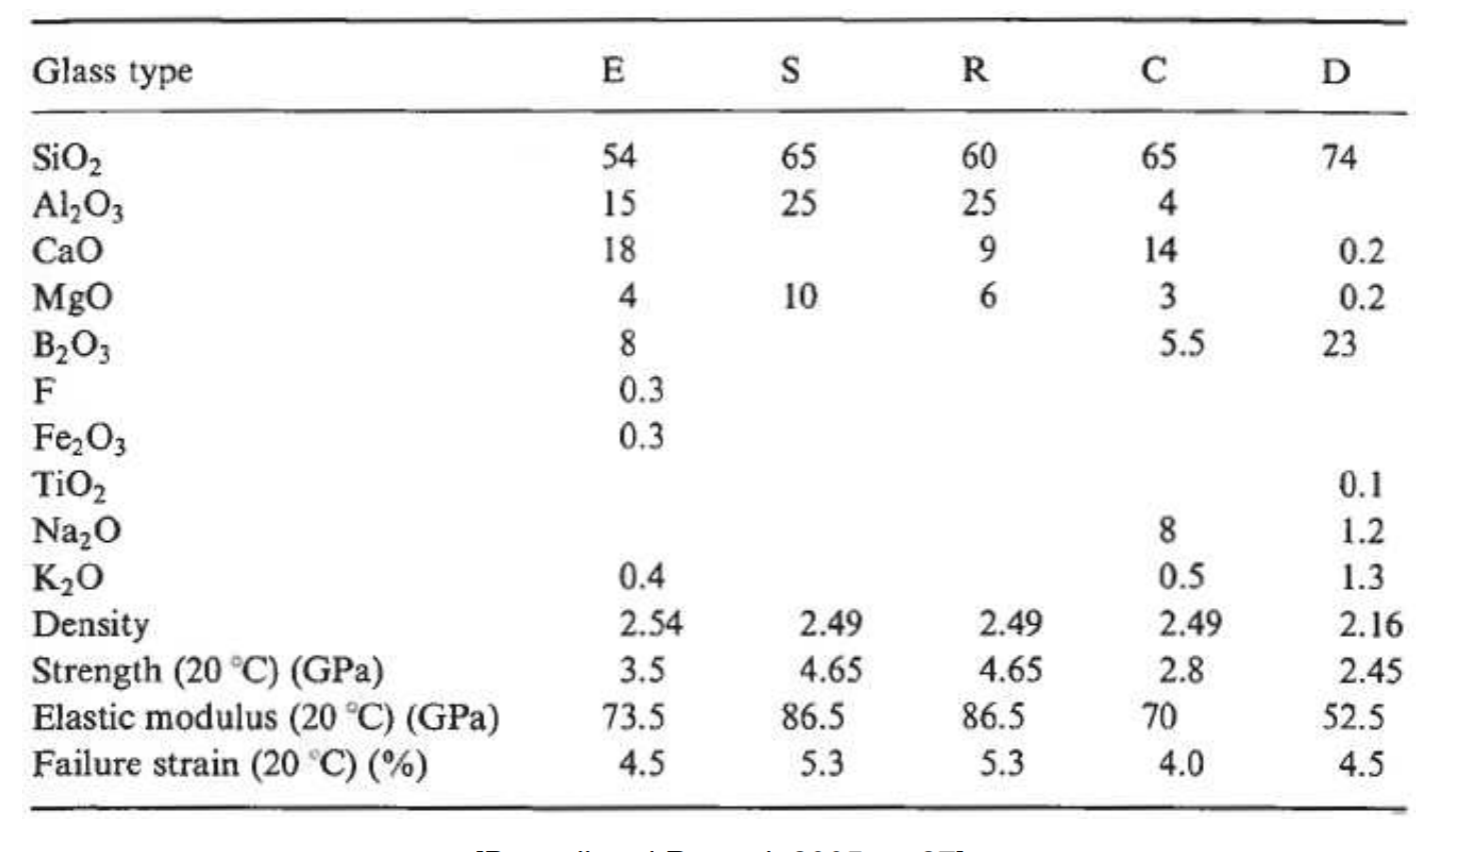
\includegraphics[width=0.8\linewidth]{./figures/glasfibertyper.png}
  \caption{Oversigt over de forskellige typer af glasfiber \citepage{bunsell2005fundamentalsfibrereinforced}{37}}
  \label{fig:glasfibertyper}
\end{figure}

\subsection{Kulfiber}
Kulfiber er typisk sort og ofte også vævet.
Disse inddeles bl.a. i følgende typer:
\begin{itemize}
  \item UHS -- Ultra-High Strength
  \item HS -- High Strength
  \item IM -- Intermediate Modulus
  \item HM -- High Modulus
  \item UHM -- Ultra-High Modulus
\end{itemize}
